In this work, we develop our generalized hierarchical Bayesian modeling framework that is able to capture the hierarchical structural relations and latent relations in the real-world recommendation scenarios. In our framework, we incorporate both user specific features and user actions into model learning so that more personalized recommendation results can be achieved. Furthermore, we present a variational inference algorithm for the HBayes framework to provide fast learning convergence.

In the following, we will describe how HBayes works by using apparel recommendation as an illustration scenario. Using a real-world example helps explain the hierarchy structural relations and latent variable conditional independence assumptions implied in HBayes. Please note that even we explain HBayes in apparel recommendation, the framework itself can be generalized into other recommendation scenarios with little modification. 



\subsection{Generative Process}

In the real-world scenario, each item or product has to come with a brand and a brand may have more than one items in the hierarchical structures. Therefore, we denote each event $t$ as a 4-tuple (Item, Brand, User, IsClick), i.e, ($\mathbf{X}_t, b_t, u_t, y_t$). $\mathbf{X}_t$ represents the item features associated with event $t$ and $y_t$ is the binary label that indicates whether user $u_t$ has clicked $\mathbf{X}_t$ or not. $b_t$ is the brand of item $\mathbf{X}_t$. 

Furthermore, we expand the hierarchy by a hidden factor, i.e., ``style''. Products from each brand $b_t$ tends to exhibit different styles or tastes, which are unknown but exsit. In this paper, brands are represented as random mixtures over latent styles, where each style is characterized by a distribution over all the items. Let $S$, $B$, $U$ and $N$ be the total number of styles, brands, users and events.

The generative process of HBayes can be described as follows:

\begin{enumerate}
\item[1.] Draw a multivariate Gaussian prior for each style $j$, i.e, $\mathbf{S}_j \sim \mathcal{N}(\mathbf{w}, \delta_s^{-1}\mathbf{I})$ where $j \in \{1, \cdots, S\}$.

\item[2.] Draw a multivariate Gaussian prior for each user $k$, i.e, $\mathbf{U}_k \sim \mathcal{N}(\mathbf{0}, \delta_u^{-1}\mathbf{I})$ where $k \in \{1, \cdots, U\}$.

\item[3.] Draw a style proportion distribution $\boldsymbol{\theta}_i$ for each brand $i$, $\boldsymbol{\theta}_i \sim \mbox{Dir}(\gamma)$  where $i \in \{1, \cdots, B\}$.

\item[4.] For each brand $i$:
	\begin{enumerate}
		\item[4.1] Draw style assignment $z_{i}$ for brand $i$, $z_{i} \sim \mbox{Mult}(\boldsymbol{\theta}_i)$.
		\item[4.2] Draw $\mathbf{B}_i \sim \mathcal{N}(\mathbf{S}_{z_i}, \delta_b)$.
	\end{enumerate}

\item[5.] For each event $t$, draw $y_t$ from Bernoulli distribution where the probability $p$ is defined as $p(y_t|\mathbf{x}_t, \mathbf{B}_{b_t}, \mathbf{U}_{u_t})$.
\end{enumerate}

\noindent where $\delta_s$, $\delta_u$ and $\delta_b$ are the scalar precision parameters and $\mathbf{w}$ is the prior mean of $\mathbf{S}_j$. 

In this work, in order to have the higher modeling flexibility and capacity, we also treat each distribution's parameter as a random variable and define hyper-priors over them. More specifically, We draw the prior mean $\mathbf{w}$ from $\mathcal{N}(\mathbf{0}, \delta_w^{-1}\mathbf{I})$. For $\delta_w$, $\delta_s$, $\delta_u$ and $\delta_b$, we define Gamma priors over them as follows: 

\begin{equation}
p(\delta_*) = \mathcal{G}(\alpha, \beta)
\end{equation}

\noindent where $\delta_* \in \{ \delta_w, \delta_s, \delta_u, \delta_b \}$. 

The family of probability distributions corresponding to this generative process is depicted as a graphical model in Figure \ref{fig:model}.

\begin{figure}[htb]
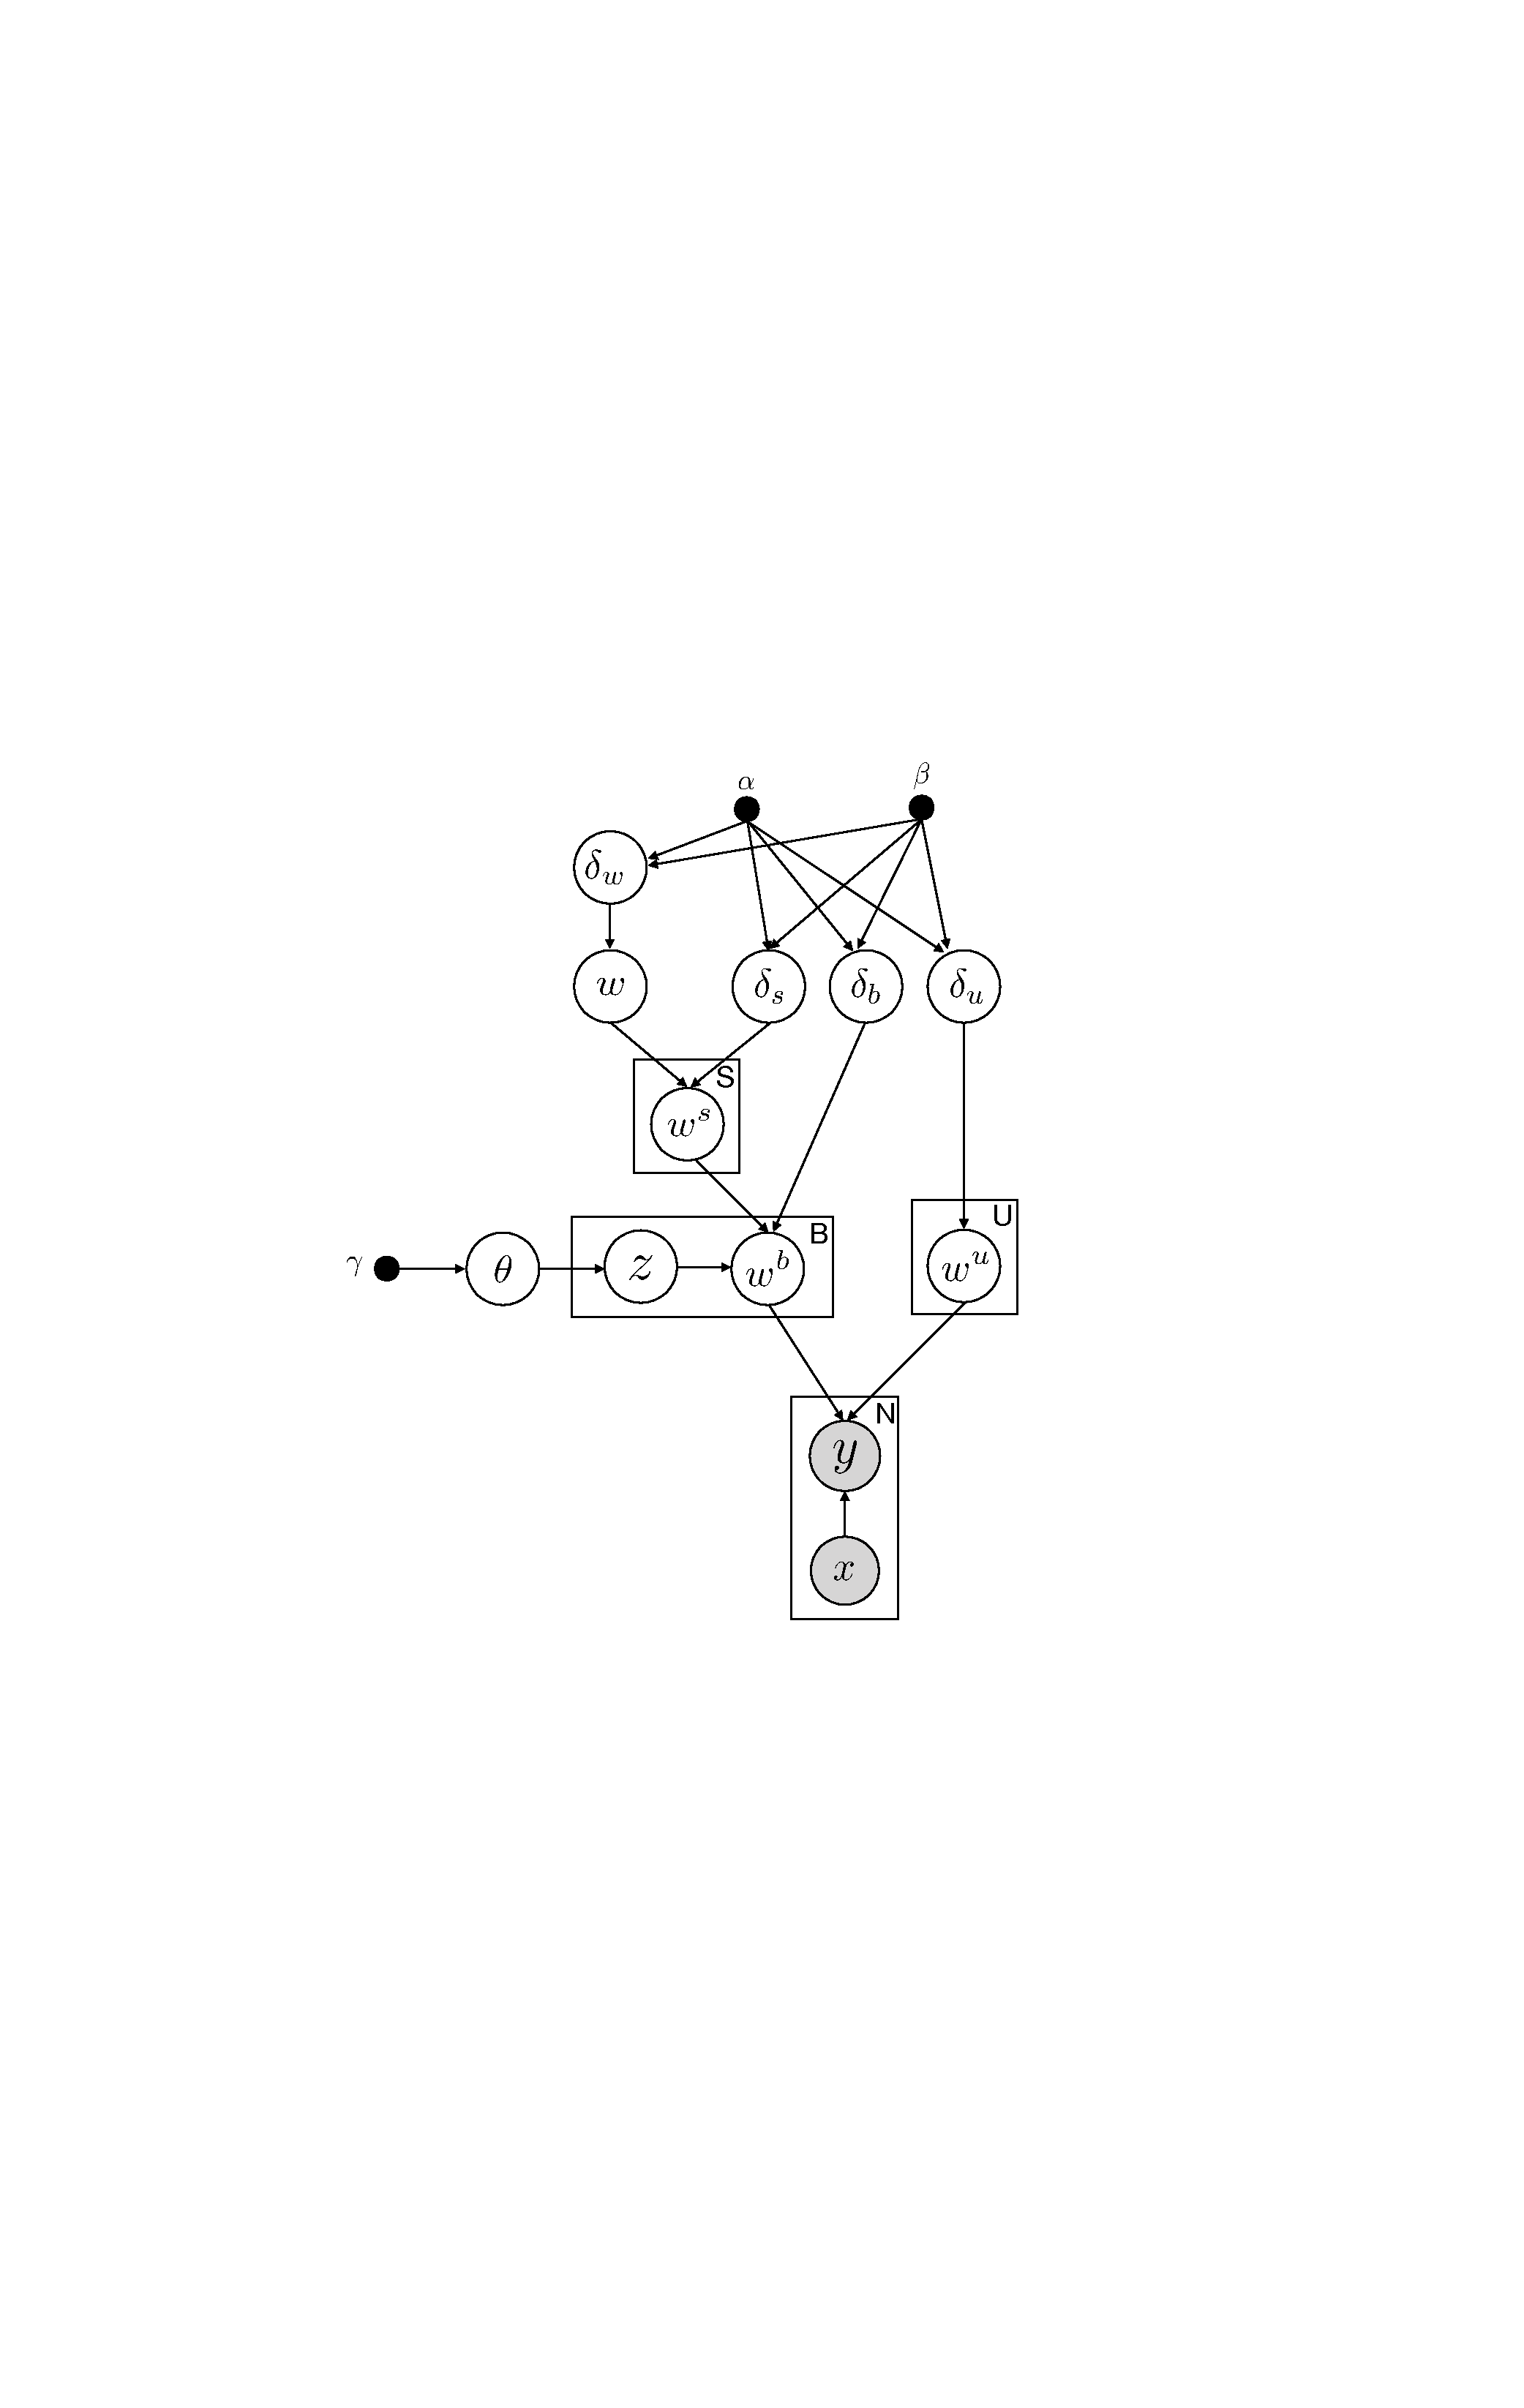
\includegraphics[width=0.8\linewidth]{fig/model}
\caption{A graphical model representation of HBayes.}
\label{fig:model}
\end{figure}

\subsection{Probability Priors \& Models}

In this work, we model the probability of a single event $t$ given ($\mathbf{X}_t, b_t, u_t, y_t$) as 

\begin{equation}
p\big(y_t|\bm{X}_t,\bm{B}_{b_t},\bm{U}_{u_t} \big)= \Big[\sigma\big(h_t\big)\Big]^{y_t} \cdot \Big[1-\sigma\big(h_t\big)\Big]^{1-y_t}
\end{equation}

\noindent where $\sigma(\cdot)$ is a logistic function, i.e. $\sigma(x)=(1+e^{-x})^{-1}$. $h_{t}\overset{\mathrm{def}}=\bm{X}_t^T(\bm{B}_{b_t}+\bm{U}_{u_t})$. $\mathbf{X}^T$ is the vector transpose of $\mathbf{X}$. $\bm{U}_{u_t}$ represents user specific information encoded in HBayes for user $u_t$ and $\bm{B}_{b_t}$ denotes the brand $b_t$'s specific information.

As mentioned in the generative process of HBayes, a brand are modeled as a random mixture over styles, which are latent variables. Hence, we model the brand parameters by a multivariate mixture Gaussian distribution defined as follows:

\begin{equation}
p(\bm{B}_i|\bm{z}_i,\bm{S}_{z_i},\delta_b) = \prod_{j}^S p(\bm{B}_i|\bm{S}_j,\delta_b)^{(\bm{z}_i=1)}
\end{equation}


Therefore, the entire events' conditional likelihood can be represented as follows:

\begin{equation}
\mathcal{L} = \prod_{t=1}^N p\big(y_t|\bm{X}_t,\bm{B}_{b_t},\bm{U}_{u_t} \big)
\end{equation}

We use $\Theta$ to denote all model parameters:

\begin{equation}
\Theta \overset{\mathrm{def}}= \Big\{\{\bm{U}_k\}, \{\bm{B}_i\}, \{\bm{S}_j\}, \bm{w}, \boldsymbol{\theta}, \delta_u,\delta_b,\delta_s,\delta_w \Big\},
\end{equation}

\noindent where $k \in \{1, \cdots, U\}$, $i \in \{1, \cdots, B\}$, $j \in \{1, \cdots, S\}$ and $\mathcal{H}$ to denote other hyper-parameters: $\mathcal{H} = \{\gamma, \alpha,\beta\}$.


The joint likelihood of the dataset $\mathcal{D}$, latent variable $\bm{Z}$ and the parameter $\Theta$ by given $\mathcal{H}$ could be written as follows:

\begin{align}
  p(\mathcal{D},\bm{Z},\Theta|\mathcal{H})= & \prod_{t=1}^N p(y_t|\bm{X}_t,\bm{B}_{b_t},\bm{U}_{u_t})  \\ 
  \cdot &  \prod_{i=1}^B p(\bm{B}_i|\bm{z}_i,\bm{S}_{z_i},\delta_b) p(\bm{z}_{i}|\bm{\theta}) p(\bm{\theta}|\bm{\gamma}) p(\delta_b) \\
  \cdot & \prod_{j=1}^S p(\bm{S}_j|\bm{w},\delta_s) p(\bm{w}|\delta_w)p(\delta_w) p(\delta_s) \\
   \cdot & \prod_{k}^U p(\bm{U}_k) p(\delta_u) 
\label{joint_p}
\end{align}






\subsection{Optimization}

\subsubsection{Inference}

\begin{equation}
p(\bm{Z},\Theta|\mathcal{D},\mathcal{H}) = \frac{p(\mathcal{D},\bm{Z},\Theta|\mathcal{H})}{p(\mathcal{D}|\mathcal{H})}
\end{equation}

In this section, we apply variational Bayes to approximate the posterior distribution $p(\bm{Z},\Theta|\mathcal{D},\mathcal{H})$ with a variational distribution $q(\bm{Z},\Theta)$, by maximizing the variational free energy defined as:
\begin{equation}
\mathcal{L}(q)= \int_\Theta \sum_{\bm{Z}} q(\bm{Z},\Theta) \log\frac{p(\mathcal{D},\bm{Z},\Theta|\mathcal{H})}{q(\bm{Z},\Theta)}d\Theta
\end{equation}

\subsubsection{Sigmoid Approximation}

\begin{equation}
\sigma(h_{i}) \geq \sigma(\xi_{i})\exp\big\{\frac{1}{2}(h_{i}-\xi_{i})-\lambda_{i}(h_{i}^2-\xi_{i}^2)\big\}
\end{equation}

$$\lambda_{i}\overset{\mathrm{def}}=\frac{1}{2\xi_{i}}[\sigma(\xi_{i})-\frac{1}{2}]$$

\noindent where $\xi_{i}$ is a variational parameter. This lower bound is derived using the convex inequality. The similar problem was discussed in \cite{jaakkola1997variational,jordan1999introduction}.

\begin{align}
& \big[\sigma(h_{i})\big]^{y_t} \cdot  \big[1-\sigma(h_{i}) \big]^{1-y_t} \\
= & \exp\big\{ y_t h_t \big\} \sigma(-h_{i}) \\
\geq & \sigma(\xi_{i})\exp\big\{y_t h_{i}-\frac{1}{2}(h_{i}+\xi_{i})-\lambda_{i}(h_{i}^2-\xi_{i}^2)\big\}
\end{align}

% \begin{equation}
% \begin{split}
% \sigma(h_{i})^{y_t} \cdot & \big[1-\sigma(h_{i})  \big]^{1-y_t} \geq \\
%  & \sigma(\xi_{i})\exp\big\{y_t h_{i}-\frac{1}{2}(h_{i}+\xi_{i})-\lambda_{i}(h_{i}^2-\xi_{i}^2)\big\}
% \label{bound}
% \end{split}
% \end{equation}



\subsubsection{Learning}

\subsection{Prediction}

\subsection{Summary}



\subsection{Relationship with Other Models}